\documentclass[10pt]{article}
\usepackage[margin=1.0in]{geometry}
\usepackage{graphicx}
\usepackage{float}
\usepackage{siunitx}
\usepackage{tabularx}
\usepackage{enumitem}
\usepackage[hidelinks]{hyperref}
\usepackage{blindtext}
\usepackage{setspace}
\usepackage{footnote}


\makesavenoteenv{tabular}

\title{
  AERSP 401B \\
  Spacecraft Design \\
  Executive Summary \\
  Reusable Lunar Surface Access Vehicle \\
}

\date{}

\begin{document}
\doublespacing

\clearpage\maketitle
\thispagestyle{empty}

\begin{center}
  
\includegraphics{SeleneSupplyLogo}\hspace*{\fill}\\  
  TEAM SELENE SUPPLY \\
  \begin{tabular}{l r}
    Team Leader: & Nicholas \textsc{Pytel} \\
    Robert \textsc{Bond} & Dominick \textsc{Allen} \\
    Michael \textsc{Croydon}  & Tyler \textsc{Meehan} \\
    Adalberto \textsc{Morales}\\
  \end{tabular}

  \hspace{1cm} \newline
  \hspace{1cm} \newline
  Instructor: Dr. David \textsc{Spencer} \\
  November 30, 2018
\end{center}

\newpage
\setcounter{page}{1}

\newpage

\section{Motivation}

The reusable Lunar Surface Access Vehicle (LSAV) has the primary
purpose of providing transportation means between the Lunar Gateway
and the lunar surface utilizing transfers from the Near Rectilinear
Halo Orbit of the gateway. This mission will provide support for
future Lunar missions and base operations by carrying both crew and
cargo too and from the surface of the moon. The mission will prove the
viability of the Lunar Gateway as a platform for future missions

\section{Mission Objectives}

In order to support lunar missions, the LSAV must satisfy the
following requirements: Must transport either crew or cargo to the
lunar surface Capable of transporting a maximum of 15 metric tons to
the surface and 10 metric tons from the surface Capable of supporting
a crew of up to four people for the duration of the mission and 24
hours on the surface.  Capable of landing anywhere (within reason) on
the lunar surface Must be reusable

These requirements are satisfied by the following major design decisions:

The LSAV will be propelled by a methane/LOx raptor engine and will be
refuelable at the lunar gateway The LSAV will support a cargo bay and
crew capsule capable of supporting the above noted requirements. The
cargo bay will provide storage space and also support a
loading/unloading crane from moving cargo to/from the surface.  The
life support system will provide moderate radiation shielding and a
breathable atmosphere during crewed operations. The Life support
system will use polycarbonate shielding as well as Lithium based CO2
scrubbers for crew support. Oxygen and water will be provided from a
small storage system separate from the propulsion system.  The
electrical system will provide power via solar panels and battery
banks. The battery banks will be capable of supplying a minimum of 36
hours of energy which will allow for operations on non illuminated
portions of the moon.  The structure will support a landing leg
assembly which will allow for landing on surfaces up to a slope of 12
degrees and free of large debris.  The LSAV will be supported by the
SpaceX ‘Starship’ launch vehicle until it reaches the Lunar Gateway
after which it will be self operating.  Refueling and resupply will
occur at the Lunar Gateway and will be supported by other NASA
missions outside the scope of this mission.

\begin{figure}[H]
  \centering
  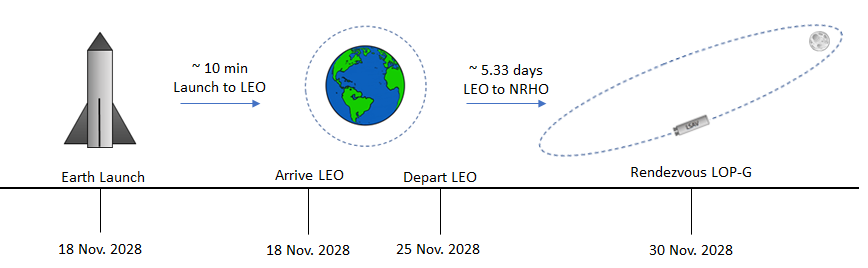
\includegraphics[width=0.9\textwidth]{toon1}
  \caption{Earth launch to LOP-G timeline}
  \label{fig:toon1}
\end{figure}

\begin{figure}[H]
  \centering
  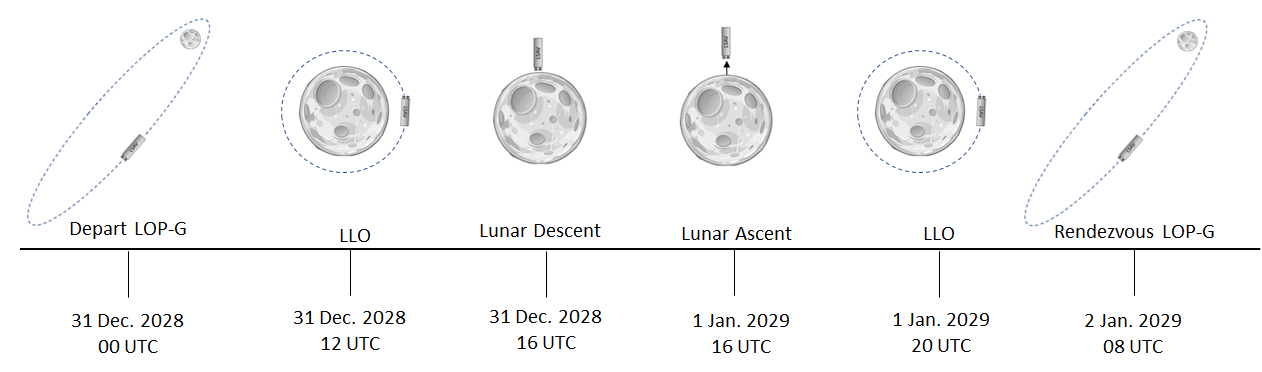
\includegraphics[width=0.9\textwidth]{toon2}
  \caption{LOP-G to lunar surface cycle timeline}
  \label{fig:toon2}
\end{figure}

\begin{table}
  \centering
  \caption{System Budgets}
  \label{table:foo}
  \begin{tabular}{lll}
    Mass (metric tons) & Power (kWhr) & Cost (USD) \\ \hline
    50 (230 wet) & 1388 & 8.1 Billion \\
  \end{tabular}
\end{table}

\section{Requirements and Constraints}

LSAV Launches from Cape Canaveral and is injected into LEO System
checkouts occur while Starship is refueled over the course of a week
Starship transfers the LSAV from LEO to NRHO and gets in close
proximity to the station Starship separates, the LSAV propulses itself
and rendezvous with the gateway.  LSAV is refueled and final system
checks occur over the course of 3 weeks Crew arrives at the lunar
gateway and the LSAV is loaded with first mission cargo LSAV departs
gateway and lands on surface Surface mission completes, LSAV launches
from surface with crew and return cargo LSAV rendezvous with lunar
gateway, crew and cargo depart and vehicles is refueled.  System
checks occur over the course of 2 weeks and any maintenance required
is completed.  Vehicle launches for next mission.  Cycle repeats for
either 30 missions or 5 years System architecture.

\section{System Descriptions}

\textbf{Structure} - The wireframe structure of LSAV will be made with
304 stainless steel tubes.  This tubing will also serve to mount the
propellant tanks and the engine.  The wireframe will be enclosed by
highly polished aluminum 6061 T6 16 gauge sheet metal which serves to
protect the insides of the vehicle but also to house the multi-layer
insulation, thermal fluid loops, wiring, and radiation shielding.

The 4 landing legs will be made with high strength carbon fiber
prepreg (symmetric twill pattern) with 350 degree Fahrenheit high
impact resistant resin.  304 stainless steel tube will make up the
components of the spring damper system and also encase the aluminum
honeycomb structure.

LSAV will be boarded and deboarded through the International Berthing
and Docking Mechanism while the cargo will be loaded through a
seperate cargo bay door.  Other mechanisms include extending and
retracting the solar panels and electric motor deployment of the
landing gear.

\textbf{Propulsion} - The tank pressurization system will use gaseous methane
and oxygen to feed the liquid propellent to the raptor engine. This
system will reduce the cost per mission by omitting the need for
helium tanks.

\textbf{ECLSS} - The crew will be housed in the front of the
spacecraft with a 6 cm polyethylene radiation shield lining the
walls. The 60 gallon water supply tank will be place in the nose cone
to also partially protect against radiation. 

\textbf{Command \& Data Handling} - The flight computer will run
VxWorks and consist of three BAE RAD5545 processors along with two
SWRI solid state recorders for storing mission data. Redundancy is
crucial for this subsystem to minimize the risk of hardware failure,
and the use of components with sufficient quality assurance
documentation reduces development and maintenance costs.

\textbf{Ground Control} - Before the LSAV has docked with the Lunar
Gateway, mission control will be at the Lyndon B. Johnson Space
Center. After docking, mission control will primarily be done at the
Lunar Gateway. The Lunar Gateway will be the primary SOCC and
POCC. The software for the various centers will custom packages that
use a mixture of existing open source and proprietary software, and
software developed in-house. Ground Control recievers will be
colocated with the Lunar Gateway's recievers.

\textbf{Communication} - The communication system has been changed to
use only S/X-Band antennae. UHF was originally going to be used for
communications between the LSAV and the Lunar Gateway, but this ended
up being too low frequency for the 80,000 km distance between the
Gateway and the LSAV. The same set of two S-Band antennae will be used
to receive communications from the Near Earth Network (NEN) and to
transmit and receive data to and from the Lunar Gateway. Additionally,
a half meter parabolic X-band antenna will be used to transmit data to
the NEN.

Total power requirements for the communications subsystem have been
reduced to 64 W, while capable of transmitting 5.5 mbps of data, and
receiving 128 kbps. This should be sufficient for receiving commands,
and sending missions informations and telemetry. More information can
be found in the link budgets in tables X. Finally, BPSK was chosen as
the modulation scheme for all communications. BPSK is chosen because
practically all NEN ground stations are capable of using it. BPSK
requires higher \(\frac{E_b}{N_o}\) compared to other modulation
schemes, but its universality makes up for this.

\textbf{Guidance, Navigation and Control} - The attitude of the LSAV
will be adjusted by a set of MR-107V engines using
hydrazine. Attitude, position, and velocity will be determined by sun
sensors, star sensors, and IMUs that are Kalman filtered by radiation
hardened RAD5545 computers. The software used to perform this will be
developed in house. During docking, LIDAR will be used to fine-tune
the approach to the International Berthing and Docking Mechanism on
the LSAV.

\textbf{Power} - The four battery banks will have their own charge
controller/monitors capable of independent operation. This will
increase the safety and reliability of the electrical system while
also providing a more stable output to the rest of the system.


The solar panels will be capable of gimbaling to allow the power input
into the system to be throttled and to match the required power. This
will mitigate the thermal burden on the thermal system by mitigating
wasted input power.

\textbf{Thermal Control Systems} - The Passive Thermal Control system
is comprised of a thick layer of multi-layer insulation held between
two walls of highly polished aluminum 6061 T6.  Highly polished
aluminum has an emissivity constant of 0.05 which makes it excellent
at radiating away the sun’s heat while also helping keep the vehicle’s
heat inside.

The Active Thermal Control system is a fluid ammonia loop with
aluminum piping mounted on the inner surface of the outer shell.  This
set-up removes any heat heat that does not get reflected and rejects
it through the heatsinks mounted on the shadowed side of the vehicle.
A simple circulation pump will run at a mass flow rate of 0.8 kg/s to
drive the loop.


\textbf{Launch Vehicle}- SpaceX BFR \& Starship will be used to carry the LSAV
to an equatorial parking orbit

Payload This system must be capable of transferring 15/10 mT of cargo
to and from the surface of the moon. Cargo is stored in the upper
portion of the LSAV so a system of cranes and sliding platforms will
be used to move this cargo. An internal crane will load cargo onto a
sliding platform which will transfer the cargo to the exterior of the
craft. Finally, an external crane will move the cargo from the
platform down to the surface of the moon, an approximately 10 m
descent, where astronauts or autonomous vehicles will be prepared to
move the cargo from the loading/unloading area.

One danger is that loading/unloading cargo from the center of mass of
the ship creates the possibility of the ship tipping over. To prevent
this, the crane will extend less than 5 m from the center of mass of
the ship, which will be within the base created by the landing
legs. As an additional precaution, the cargo will be divided into
parcels small enough to keep any tipping moment within a safe
margin. This safe margin will be based on the moments of inertia of
the ship at landing.


\newpage

\section{Appendix}

\begin{table}[H]
  \centering
  \caption{Subsystem Costs}
  \begin{tabular}{p{2in}r} 
    Subsystem Cost & Estimate (Millions of USD) \\ \hline
    Launch Vehicle & 200 \\
    Propulsion & 400 \\
    Ground Control & 100 \\
    Structures & 600 \\
    Communications & 10 \\
    C\&DH & 100 \\
    GNC & 200 \\
    Power & 120 \\
    Thermal & 40 \\
    Payload & 30 \\
    ECLSS & 800 \\ \hline
    Integration, Integration Testing \& Qualification & 5500 \\ \hline
    Total & 8100 \\
  \end{tabular}
\end{table}

\begin{table}[H]
  \centering
  \caption{Link Budget for LSAV to Gateway}
  \label{table:linkbudgetlsav}
  \begin{tabular}{lrr}
    {} & LSAV to Gateway &Gateway to LSAV \\ \hline

    Transmit Power (P)&24 W&45W \\

    Line  Loss \((L_l)\)&-1 dB&-1 dB \\
    Transmit Gain \((G_t)\)&25 dB&35 dB \\
    Space Loss \((L_s)\)&-197.6 dB&-197.6 dB \\
    Path Loss \((L_a)\)&0 dB&0 dB \\
    Receiving Gain \((G_r)\)&30 dB&30 dB \\
    System Temperature Noise \((T_s)\)&27.9 dB&27.9 dB \\
    Data Rate (R)&512 kbps&128 kbps \\
    Implementation Loss \((L_i)\)&-2 dB&-2 dB \\
    Estimated \(\frac{E_b}{N_o}\)&11.9 dB&30.6 dB \\
    Required \(\frac{E_b}{N_o}\)&8.5 dB&10.5 dB \\
    Link Margin&3.4 dB&20.1 dB \\

  \end{tabular}
\end{table}

\begin{table}[H]
  \centering
  \caption{Link Budget for LSAV to NEN}
  \begin{tabular}{lrr}
    &LSAV to NEN&NEN to LSAV \\ \hline 
    Transmit Power (P)&40 W&200 W \\
    Line  Loss \((L_l)\)&-1 dB&-1 dB \\
    Net Transmit Gain* \((G_t)\)&29.5 dB&44.8 dB \\
    Space Loss \((L_s)\)&-224.9 dB&-212.9 dB \\
    Path Loss \((L_a)\)&-1 dB&-1 dB \\
    Receiving Gain \((G_r)\)&61.7 dB&30 dB \\
    System Temperature Noise \((T_s)\)&27.9 dB&27.9 dB \\
    Data Rate (R)&5 mbps&128 kbps \\
    Implementation Loss \((L_i)\)&-2 dB&-2 dB \\
    Estimated \(\frac{E_b}{N_o}\)&12 dB&30.6 dB \\
    Required \(\frac{E_b}{N_o}\)&8.5 dB&10 dB \\
    Link Margin&3.5 dB&20.6 dB \\
  \end{tabular}
\end{table}

\begin{table}[H]
  \centering
  \caption{Table of subsystem mass}
  \label{table:mass_summary}
  \begin{tabular}{lr} \hline
    Subsystem & Mass (kg) \\ 
    Structure & 15,000 \\ 
    Launch Vehicle & N.A. \\ 
    Propulsion & 177500 \\
    Ground Control & N.A. \\
    Communications & 25 \\
    C\&DH & 100 \\
    GNC & 260 \\
    Power & 3850\\
    Thermal & 1000 \\
    ECLSS & 3500 \\ 
    Total & 201000 \\ 
  \end{tabular}
\end{table}

The volume estimate table provides a rough estimate of the total
volume each subsystem will use on the LSAV. The structure subsystem
volume includes the cargo bay.

\begin{table}[H]
  \centering
  \caption{Table of subsystem volume}
  \label{table:volume_summary}
  \begin{tabular}{lr} \hline
    Subsystem & Volume ($m^3$) \\ 
    Structure & 800 \\ 
    Launch Vehicle & N.A. \\ 
    Propulsion & 200 \\
    Ground Control & N.A. \\
    Communications & 1 \\
    C\&DH & 1 \\
    GNC & 1 \\
    Power & 3 \\
    Thermal & 6 \\
    ECLSS & 75 \\  
  \end{tabular}
\end{table}

The subsystem power chart breaks down the max instantaneous power
consumption rate of each subsystem. Some subsystems, such as ECLSS and
Thermal, will have a relatively consistent power consumption rate
while others, such as Payload and Propulsion, will be intermittent and
likely use very little of the available energy in the batteries. The
total energy estimate was based on the worst case scenario of max
power consumption from each subsystem for a total of 36 hours.

\begin{table}[H]
  \centering
  \caption{Table of subsystem power}
  \label{table:P}
  \begin{tabular}{p{2in}r} 
    Subsystem & Power (kw) \\ \hline
    Structure & 2 \\ 
    Launch Vehicle & N.A. \\
    Propulsion & 1 \\
    Thermal & 5.50 \\
    GNC & .2 \\
    Payload & 1 \\
    C\&DH & .200 \\
    Structures \& Mechanisms & 2 kW \\
    Ground Control & N.A. \\
    Launch Vehicle & N.A. \\ \hline
    Maximum Instantaneous Power Consumption & 12.4 kW \\ \hline
    Total Energy Required & 1380 kWh \\ 
  \end{tabular}
\end{table}


Power

The battery bank controllers will each be capable of independent
control and will be interfaced with each other and the main LSAV
control system. This will allow fine tuning of power input/output of
each battery bank based on proximity to the load. It will also allow
for fast countermeasures to take place in the event of a critical
battery failure by keeping the control system local to the individual
battery bank.

The solar cell arrays will be capable of adjusting their solar flux
exposure by changing their angle relative to the solar radiation
source. This will mitigate the use of radiative power dissipation
systems in the event that the system has fully charged batteries and
is generating more power than the LSAV requires. In addition to
mitigating solar flux input, it can also be used to maximize flux
input when solar flux is not normal to the cell arrays. This will
allow maximum energy harvesting which will allow for more power usage
during missions (if needed).

\textbf{Structures and Mechanical Systems} 
	\textbf{Wireframe Structure}	The wireframe structure of LSAV will be made with a 301 stainless steel, wireframe, round tube structure.  301 is chosen because it is cheaper than 316 and has a higher endurance limit and yield strength than 304. Endurance limit and yield strength of 301 are 38 ksi and 74 ksi respectively. Stainless is also very good for supporting the cryogenic LOX tank due to the fact that its tensile strength increases at lower temperatures.  Round tube is chosen because it is easy to bend into the circular structure shape

Weight and cost estimate using twelve 2” diameter, 0.375” wall thickness tubes for vertical supports with an assumed max force seen during launch (Starship acceleration approximately 2.5 g’s) and a factor of safety (F.O.S.) of 1.2.
\begin{enumerate}
\item Price = \$21.00 per pound

\item Total weight  = 4600 lbs = 2 MT

\item Total material cost = \$97000
\end{enumerate}

The inner and outer panels of the wire frame will be made out of  highly polished Aluminum 6061 T6.  Aluminum 6061 has good weldability and formability for manufacturing and excellent corrosion resistance which is need for the long term use of the craft.  It also has a high tensile strength to add to the strength of the wire frame. It maintains sufficient strength at the temperatures it will experience on the moon as well (414 MPa @ -200 C, 310 MPa @ 24 C and 234 MPa at 150 C)

Weight and cost estimate using 18 gauge Aluminum 6061 T6 sheets:
\begin{enumerate}
		\item Price = \$5.50 per ft\textsuperscript{2}
		\item Total weight = 400 kg
		\item Total material cost = \$20000 
\end{enumerate}


\textbf{Ground Control} - The decision to use a mixture of existing
proprietary and open source software in addition to new in-house
software was made on the basis that although many solutions exist,
some new code will have to be developed to handle situations that are
particular to the LSAV.

\textbf{GNC} - The decision to use in-house developed software was
made on the basis that integrating the software for the sensor suites
and controlling the thrusters will be a unique challenge. 

\end{document}